\begin{quote} \textit{1) Estudiar las corrientes y tensiones en todos los componentes en función del tiempo, desde que se enciende el regulador ($t=0$) hasta régimen permanente. En particular, en régimen permanente, estudiar en detalle las corrientes y tensiones en un intervalo de unos pocos periodos.}
\end{quote}

\HgraficarPNG{0.4}{fly}{Regulador \textit{Flyback} aislado.}{fig:cto}

	En la Figura \ref{fig:cto} se muestra el circuito completo bajo análisis. Se trata de un regulador tipo \textit{Flyback} aislado utilizado a nivel industrial ya que posee múltiples salidas y los componentes magnéticos que lo conforman son económicos.\\
\indent Para realizar un análisis cualitativo del mismo, se puede considerar el circuito simplificado de la Figura \ref{fig:cto_simple}, donde se reemplazó el rectificador por una tensión constante, y sólo se consideró una de las salidas.

\HgraficarEPS{0.5}{fly_simple}{Circuito simplificado.}{fig:cto_simple}

\begin{itemize}
	\item \textcolor{blue}{\textbf{Primer ciclo:}} $V_{GS}=\SI{12}{\volt}$ (llave cerrada) el MOSFET se encuentra en conducción, por lo que $L_1$ se carga e induce una tensión en $L_2$, de polaridad inversa según la notación de los bornes homólogos. Esto hace que el diodo $D$ esté en inversa y por ende no circule corriente por la malla de $L_2$. En esta parte del ciclo ambos núcleos almacenan energía.

	\item \textcolor{red}{\textbf{Segundo ciclo:}} $V_{GS} = \SI{0}{\volt}$ (llave abierta) la tensión en $L_1$ se inveirte para contrarrestar el cambio abrupto de corriente, por lo que también se invierte la polaridad en $L_2$, pero la corriente en $L_1$ será nula por estar el MOSFET en corte.
		En este ciclo $L_2$ se descarga con el fin de cargar al capacitor $C_S$, el cuál se encarga de entregar la tensión de salida. A su vez se sabe que el circuito está operando en modo discontinuo, por lo que $L_2$ alcanza a descargase por completo en este ciclo.
\end{itemize}


	Asimismo se debe destacar que $L_1$ y $L_2$ no conforman un transformador sino que son dos inductores porque no circula corriente por ambos inductores simultáneamente.

\begin{figure}[H]
	\centering
	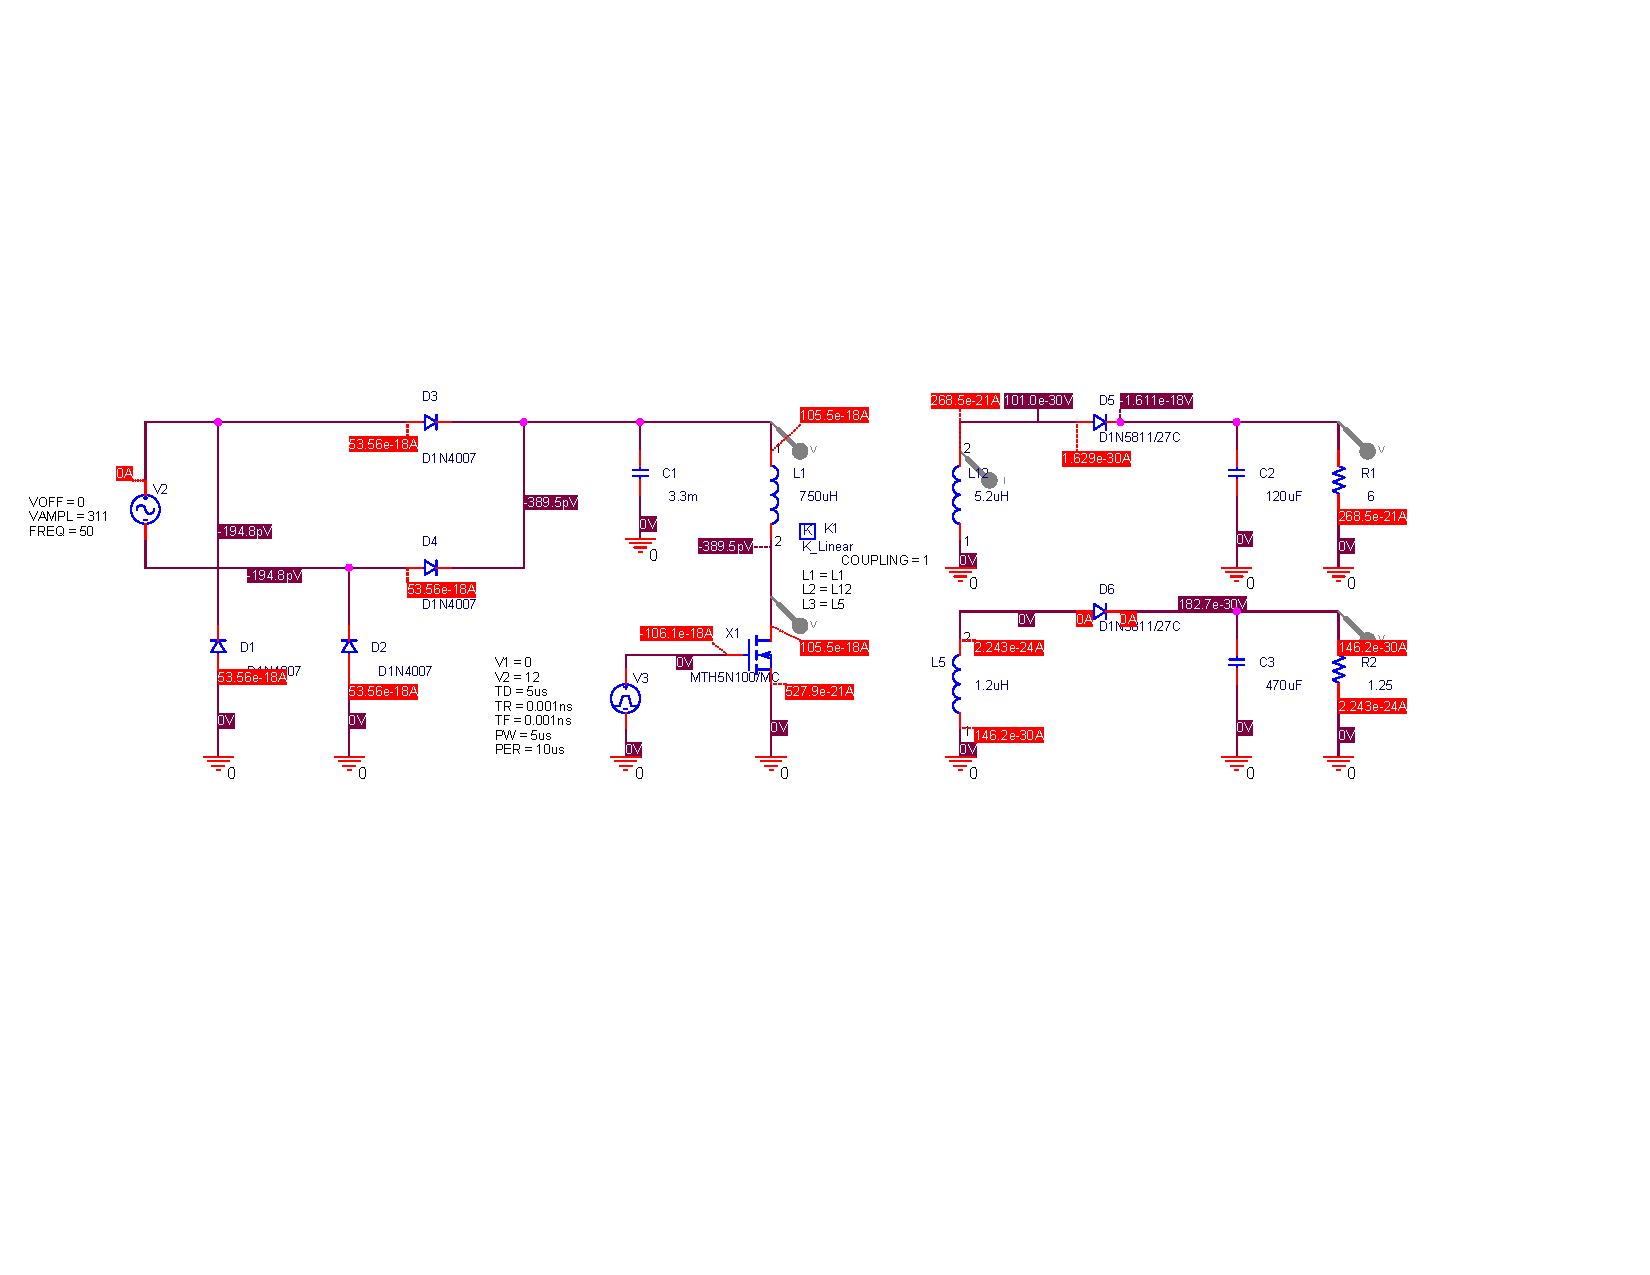
\includegraphics[scale=0.5]{Figuras/1_esquematico.pdf}
	\caption{Circuito bajo análisis con \textit{PSpice}.}
	\label{fig:esq}
\end{figure}

	En la Figura \ref{fig:esq} se muestra el esquema de simulación, siendo las corrientes y tensiones más relevantes las que se muestran en \ref{fig:transitorio}{ y \ref{fig:permanente}. Se consideró como señal de entrada la máxima posible, \SI{220}{\volt} @ \SI{50}{\hertz}. Por otra parte la señal de pulso elegida posee un ciclo de trabajo \num{0,5} y frecuencia de conmutación de \SI{100}{\kilo\hertz}. La simulación se realizó desde $t=0$ hasta \SI{10}{\milli\second} observando que luego de \SI{5}{\milli\second} se logra la estabilización del circuito. Las tensiones de salida obtenidas resultaron de aproximadamente \SI{10.5}{\volt} y \SI{25}{\volt}.
	A su vez como toda fuente conmutada la tensión de salida presenta rizado, el cuál puede aprecierse con más detalle en las Figuras \ref{fig:permanente}, siendo el valor de rizado para cada caso:
	$$\Delta V_{o1} \simeq \SI{88}{\milli\volt} $$
	$$ \Delta V_{o2} \simeq \SI{200}{\milli\volt} $$

	Se corrobora que el conversor se encuentra operando en modo discontinuo con $D=\num{0,5}$ debido a las formas de onda de la corriente en $L_{12}$, $T>t_{carga}+t_{descarga}$, es decir que el inductor se descarga por completo en cada ciclo. El modo discontinuo también se evidencia en la forma de tensión de \textit{drain} del MOSFET (nodo de conmutación), aunque no se logre apreciar en el gráfico posee la forma \ref{fig:v_drain}


\HgraficarPNG{0.3}{v_drain}{Tensión de \textit{drain}}{fig:v_drain}


\begin{figure}[H]
	\centering
	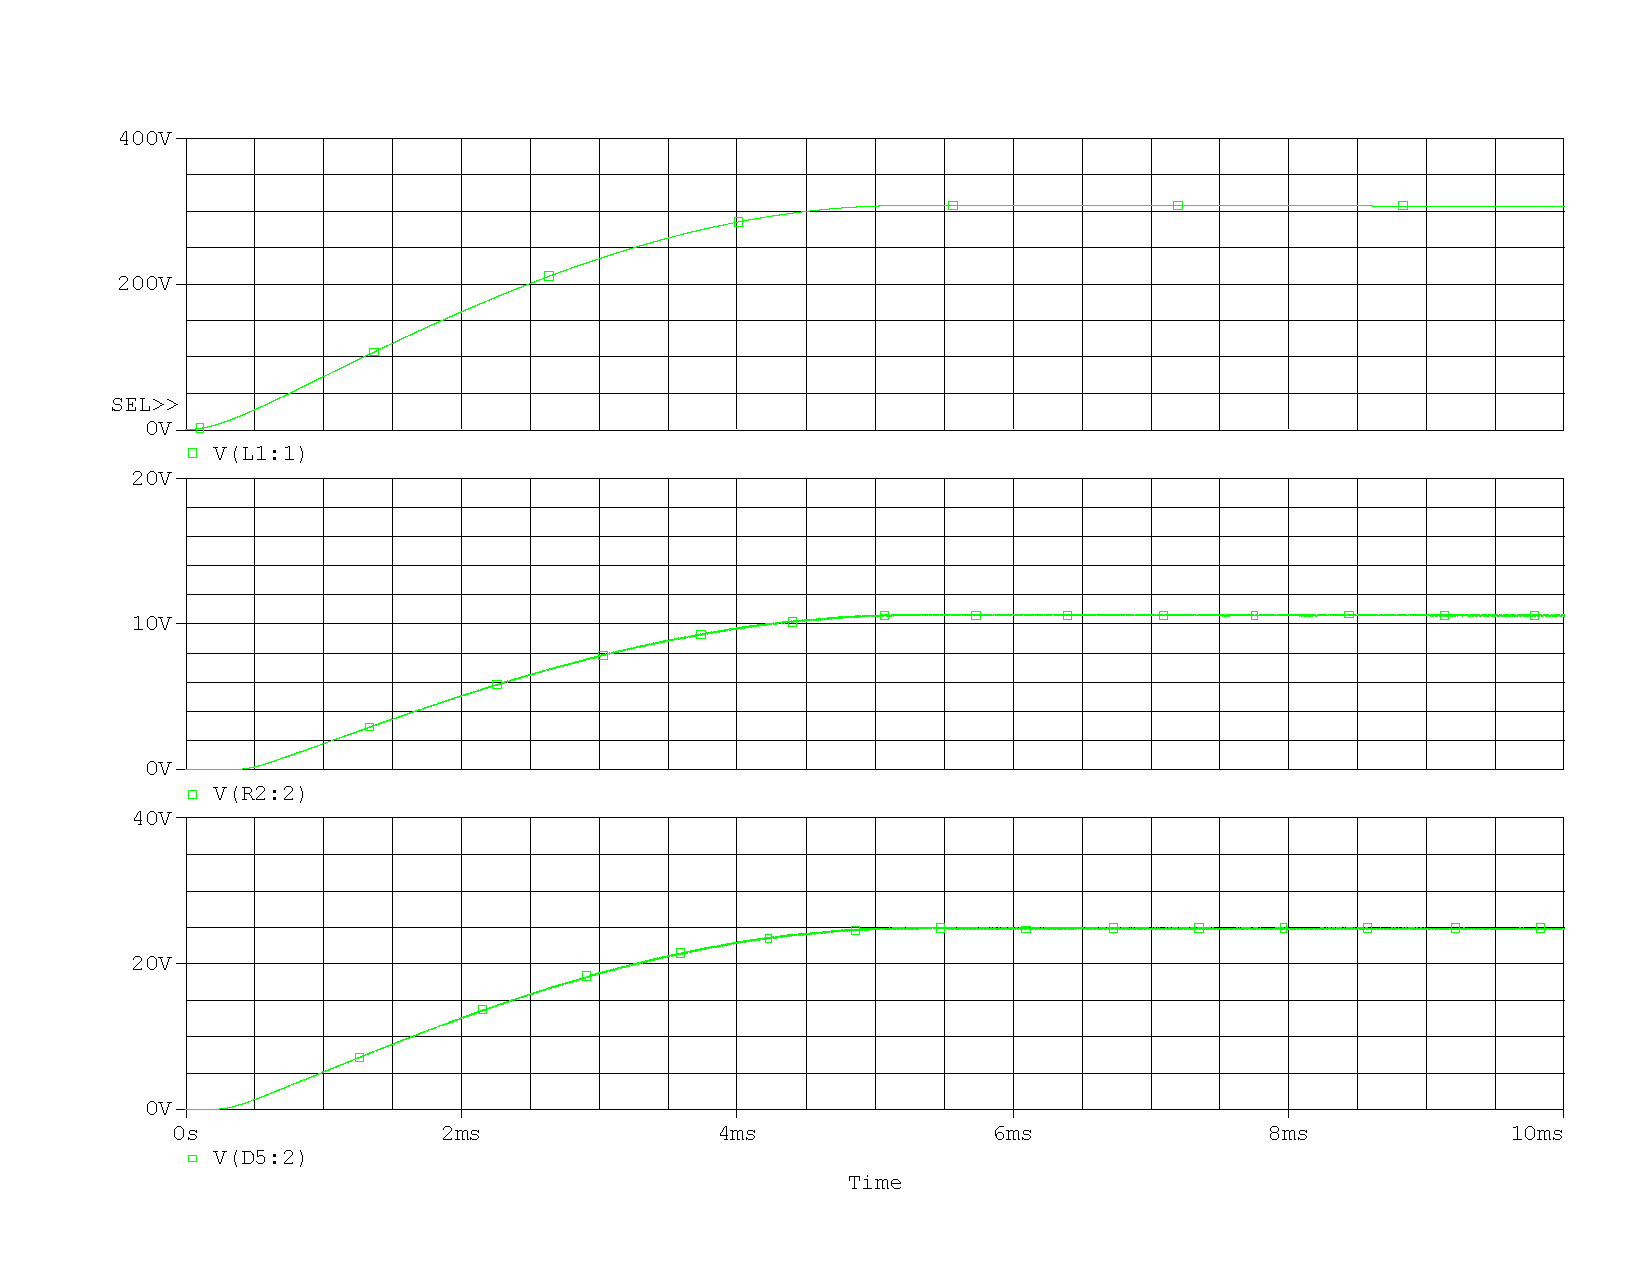
\includegraphics[scale=0.5]{Figuras/1_transitorio_con_rectificador.pdf}
	\caption{Transitorio.}
	\label{fig:transitorio}
\end{figure}

\begin{figure}[H]
	\centering
	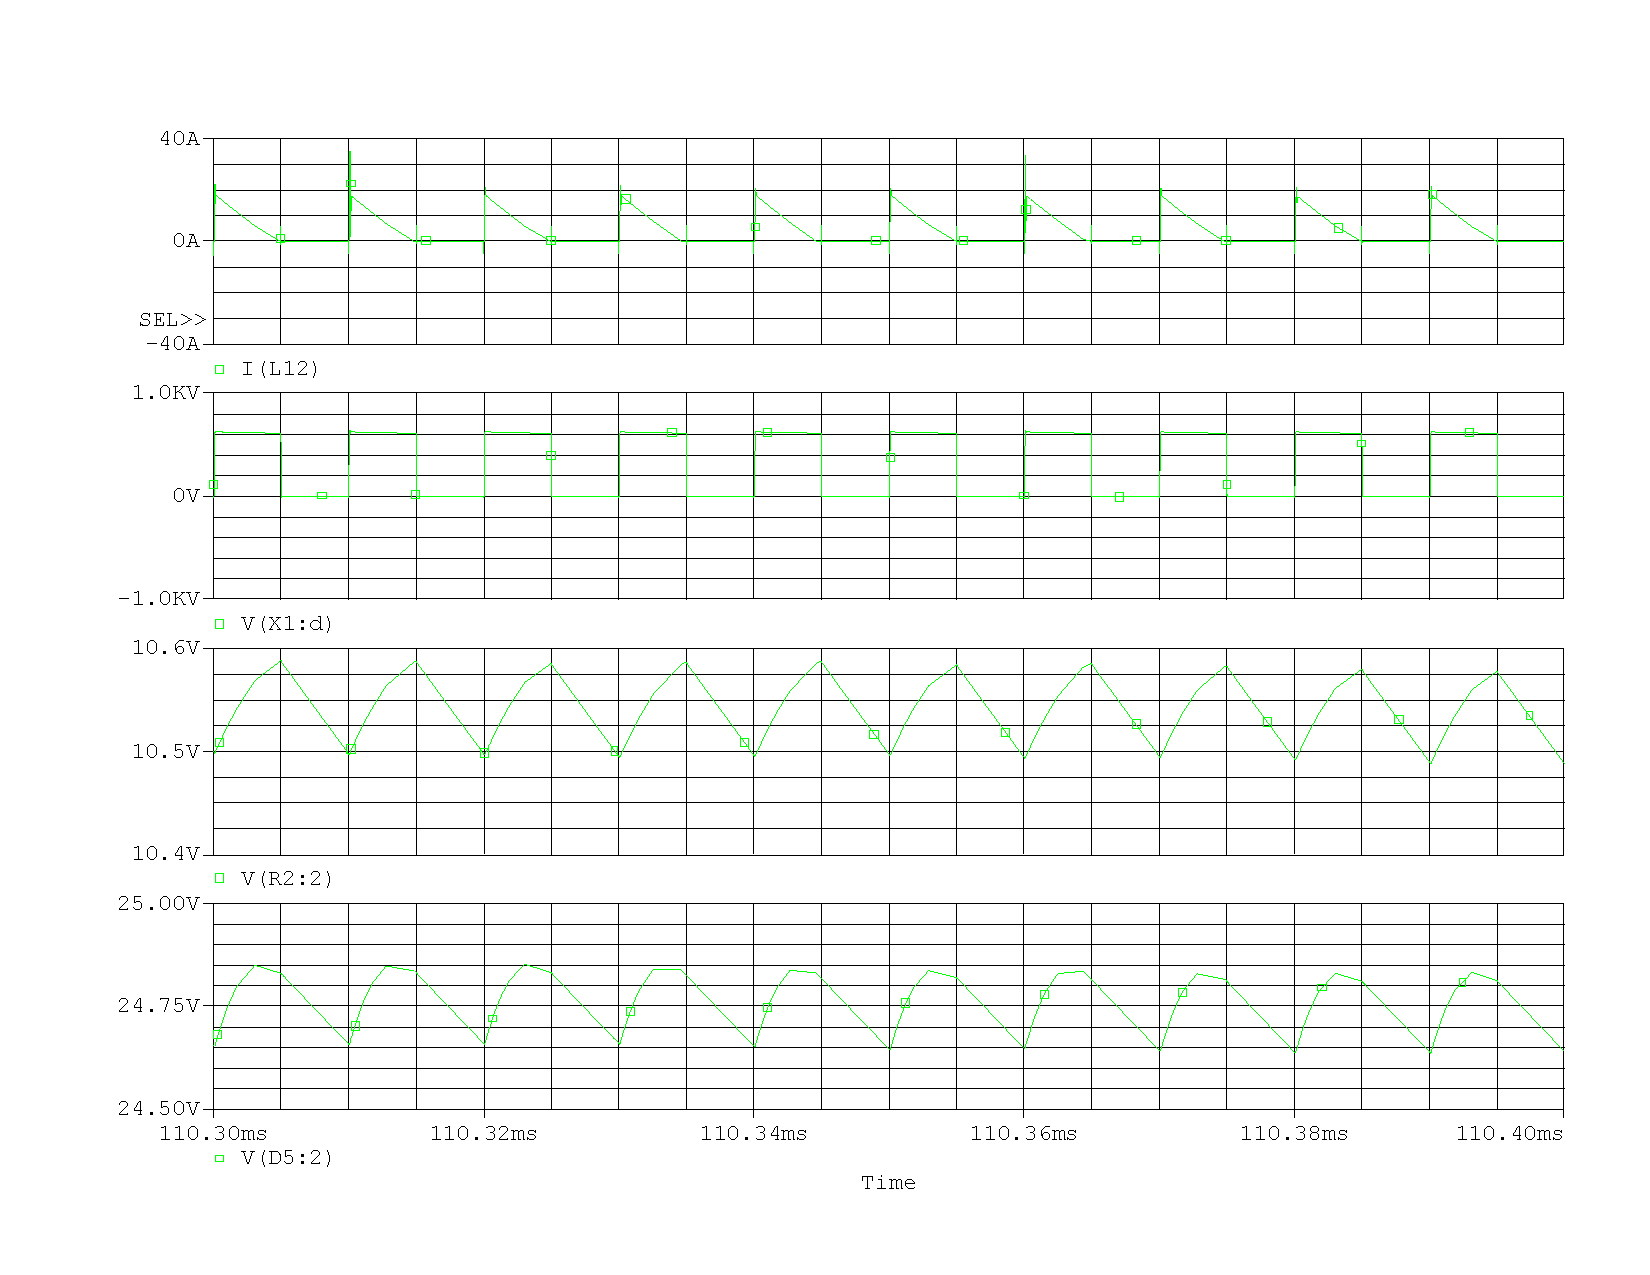
\includegraphics[scale=0.5]{Figuras/1_regimen_permanente.pdf}
	\caption{Régimen permanente.}
	\label{fig:permanente}
\end{figure}


